\documentclass{article}

\usepackage[english]{babel}
\usepackage[letterpaper, top=2.5cm, bottom=2.5cm, left=2.5cm, right=2.5cm, marginparwidth=1.75cm]{geometry}

\usepackage{amsmath,amsthm,amssymb}
\usepackage{bbold}
\usepackage{graphicx}
\usepackage{listings}
\usepackage{multicol}
\usepackage{setspace}
\usepackage{enumitem}
\usepackage{float}
\usepackage{apacite}
% Common set symbols
\newcommand{\Z}{\mathbb{Z}}
\newcommand{\N}{\mathbb{N}}
\newcommand{\R}{\mathbb{R}}
\newcommand{\Q}{\mathbb{Q}}
\newcommand{\C}{\mathbb{C}}
\newcommand{\B}{\mathbb{B}}
\newcommand{\nullset}{\varnothing}
\newcommand{\powerset}[1]{\mathcal{P} ({#1})}
\newcommand{\ol}[1]{\overline{#1}}

\newcommand{\divides}{\mid}
\newcommand{\notdivides}{\nmid}

\newcommand{\st}{\text{ such that }}
\newcommand{\pmi}{\text{ principle of mathematical induction }}

\newcommand{\nitem}[1] % sets enumerate to a specific number {arg1}
{
    \setcounter{enumi}{#1}
    \addtocounter{enumi}{-1}
    \item
}
\usepackage{multicol}
\newtheorem{theorem}{Theorem}[section]
\newtheorem{lemma}{Lemma}[section]
\title{U-Soar 2025 Summary}
\author{
    Micah Sherry \\
    \texttt{nbzx@iup.edu}
    \and
    Dr. Francisco Alarcon\\
    \texttt{falarcon@iup.edu}
}

\begin{document}

    \maketitle

    \begin{abstract}
        The Boolean semifield, denoted as $\B$, is an algebraic structure with two operations: logical OR, analogous to addition, and
        logical AND, analogous to multiplication. Our research explores the factorization of polynomials over the Boolean semifield, denoted as $\B[x]$.
        
        A key challenge in $\B[x]$ is that factorization is not unique. Specifically, we investigate the factorization of a particular
        class of polynomials in $\B[x]$ namely: $$f_n(x) = \sum_{i=0}^{n} x^i = x^n + x^{n-1} + \cdots + x + 1$$
        
        Understanding the non-unique factorization of these polynomials is a central focus of our study. This research contributes to a
        deeper understanding of algebraic structures beyond traditional fields and rings.
    \end{abstract}

    \section{Definitions}
        Let $\B$ be the Boolean semifield, $\B = \{0, 1\}$  equipped with two binary operations logical OR (+) which is analogous to addition and logical AND (·)
        which is analogous to multiplication. And let $\B[x]$ be the set of all polynomials over this semifield.
        We define a specific polynomial $f_n(x)$ as the sum of powers of $x$ from $0$ to $n$, which can be written as 
            $f_n(x) = \sum_{i=0}^n x^i = x^n + x^{n-1} + \dots + x + 1 \in \B[x]$.
        Furthermore, we introduce an isomorphism $\theta(f(x))$ that maps polynomials from $\mathbb{B}[x]$ to Numbral arithmetic
        (described in the paper 'On the Sequence A079500 and Its Combinatorial Interpretations'),
        with $\theta^{-1}(n)$ being its inverse. Notably, the isomorphism $\theta(f(x))$ is equivalent to evaluating the polynomial at $x=2$,
        expressed as $\theta(f(x)) = [f(2)]$, where $[n]$ represents the base 2 representation of an integer $n$.

    \section{Factorizations of the form $(x+1)h(x)$}
        Let $G_n$ be the set of $g(x) \in \B[x]$ such that $g(x) = \sum_{i=1}^n a_ix^i$
        and for all $a_i$ if $a_i = 0$ then $a_{i+1}\neq 0$.
        Let $F(n)$ = the nth Fibonacci number.

    \begin{theorem}
        $|G_n| = F(n+2)$
    \end{theorem}
    \begin{proof}
        The proof will be by strong induction
            \subsubsection*{\textbf{Base Cases:}}
            \begin{itemize}
                \item $n=1$; $G_1 =\{1x, 0x\}$; $|G_1|= 2 = F(3)$
                \item $n=2$; $G_2 =\{1x^2 + 1x, 1x^2 + 0x, 0x^2 + 1x \}$; $|G_2|= 3 = F(4)$
            \end{itemize}
            Therefore the base cases hold.
            \subsubsection*{\textbf{Induction Hypothesis:}}
                Assume that $|G_j| = F(j+2)$ for all $j \in \{1, 2, \ldots, k\}$ for some $k$.
            \subsubsection*{\textbf{Inductive Step:}}
                Let $g(x) \in G_{k+1}$. Consider the cases for $a_{k+1}$.
                \begin{enumerate}
                    \item Case 1. $a_{k+1} = 1$. In which case the rest of the polynomial can be any polynomial in $G_k$.
                    \item Case 2. $a_{k+1} = 0$ which implies $a_k = 1$. In which case the rest of the polynomial can be any polynomial in $G_{k-1}$.
                \end{enumerate}
                So, $G_{k+1} = G_k + G_{k-1} = F_{k+2} + F_{k+1} = F_{k+3}$. Therefore, by the Principle of Mathematical Induction $|G_n| = F_{n+2}$.
    \end{proof}

    \begin{theorem}
        $(x+1)h(x) = f_n(x)$ if and only if $h(x) = x^{n-1} + g'(x)+1$ where $g'(x) \in G_{n-2}$.
    \end{theorem}
    \begin{proof}
        ($\rightarrow$): Assume that $(x+1)h(x) = f_n(x)$ and let $h(x) = \sum_{i=0}^{n-1} a_i x^i$.
        (Notice $a_{n-1} = a_0 = 1$ otherwise it would contradict the assumption). Now assume
        for the sake of contradiction that there exists $k < n-1$ such that $a_k = a_{k+1} = 0$.
        Consider the following:
        $$(x+1)h(x) = x \sum_{i=0}^{n-1} a_i x^i + \sum_{i=0}^{n-1} a_i x^i.$$
        Notice the $(k+1)^{\text{th}}$ term will have coefficient $a_k + a_{k+1} = 0$,
        contradicting the original assumption.

        ($\leftarrow$): Assume $h(x) = \sum_{i=0}^{n-1} a_i x^i$ with $a_{n-1} = a_0 = 1$ and for
        all $a_i$, if $a_i=0$ then $a_{i+1} \neq 0$. Consider the following:
        $$(x+1)h(x) = \sum_{i=0}^{n-1} a_i x^{i+1} + \sum_{i=0}^{n-1} a_i x^i = a_{n-1}x^n + \sum_{i=1}^{n-1}(a_{i-1}+a_i)x^i + a_0 = f_n(x).$$
        Therefore, the theorem holds.
    \end{proof}

    \begin{theorem}
        There are $F(n)$ polynomials $h(x)$ such that $(x+1)h(x) = f_n(x)$.
    \end{theorem}
    \begin{proof}
        Consider the following cases:
        \begin{itemize}
            \item $n = 1$. $h(x) = 1$ is the only valid $h(x)$ such that $(x+1)h(x) = f_1(x)$.
            So, the theorem holds in this case.
            \item $n = 2$. $h(x) = x+1$ is the only valid $h(x)$ such that $(x+1)h(x) = f_2(x)$.
            So, the theorem holds in this case.
            \item $n \geq 3$. In this case, the theorem follows directly from the two previous theorems.
        \end{itemize}
    \end{proof}

    \section{Divisibility Conditions for $f_n(x)$}
    \begin{lemma}
        Lemma 3.1 from the paper 'On the Sequence A079500 and Its Combinatorial Interpretations'
        states conditions for divisibility in the numbral arithmetic: For each $n, d > 0$,
        it holds that $[d]$ is a divisor of $[2^n - 1]$ if and only if it ends with the digit 1,
        and it does not contain any subsequence of 0s having length greater than $n-k$, with $k$
        being the length of $[d]$.
    \end{lemma}

    \begin{theorem}
        If $2k - 1 \leq n$ then $x^k + 1$ divides $f_n(x)$.
    \end{theorem}
    \begin{proof}
        Assume $2k - 1 \leq n$ and let $d = \theta(x^k + 1) = 10 \cdots 01$ (notice $[d]$ is
        length $k+1$ and has $k-1$ zeros). Notice $\theta(f_n(x)) = 2^{n+1} - 1$. By the
        above lemma, $d$ divides $[2^{n+1} - 1]$ because $k-1 < n+1-(k+1)$, which is
        equivalent to $2k-1 \leq n$. And by applying $\theta^{-1}$ we see $x^k+1$ divides $f_n(x)$.
    \end{proof}

    \begin{theorem}
        Let $g(x) \in \B[x]$ such that the constant term of $g(x)$ is 1. If $\deg(g(x)) = k$
        and $2k-1 \leq n$, then $g(x)$ divides $f_n(x)$.
    \end{theorem}
    \begin{proof}
        Assume $2k-1 \leq n$ and let $d = \theta(g(x))$ (notice $[d]$ is length $k+1$). Let $m$ be
        the maximum length of zeros in $[d]$. Notice $m \leq k-1$. Notice $\theta(f_n(x)) = 2^{n+1}-1$.
        By the above lemma, $d$ divides $2^{n+1}-1$ because $k-1 \leq n+1-(k+1)$, which is
        equivalent to $2k-1 \leq n$. And by applying $\theta^{-1}$ we see $g(x)$ divides $f_n(x)$.
    \end{proof}
    \pagebreak
    \section{Number of unique Factorizations of $f_n$}
    Since Factorization in $\B[x]$ is not unique an interesting question is how many  unique factorizations are there for a given polynomial?
    we looked at factorizations for the class of polynomials $f_n(x)$.
    One of the challenges of this is that factoring in $\B[x]$ is an NP-complete problem.
    This caused us only to be able to run the factorization algorithm for low values of $n$.
    \begin{figure}[h!]
        \centering
        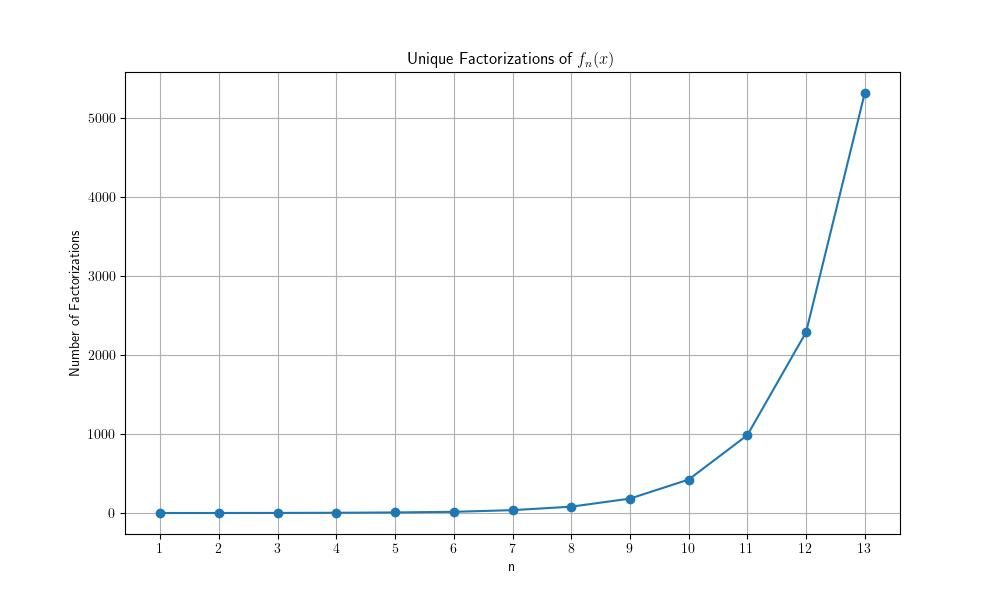
\includegraphics[width=0.75\textwidth]{factorization.jpg}
    \end{figure}
    \\
    We also looked at the ratio at which the number of factors increases. The ratio seemed to approach 2.32.
    More work is needed to see if this trend continues as $n$ increases.
    \begin{figure}[h!]
        \centering
        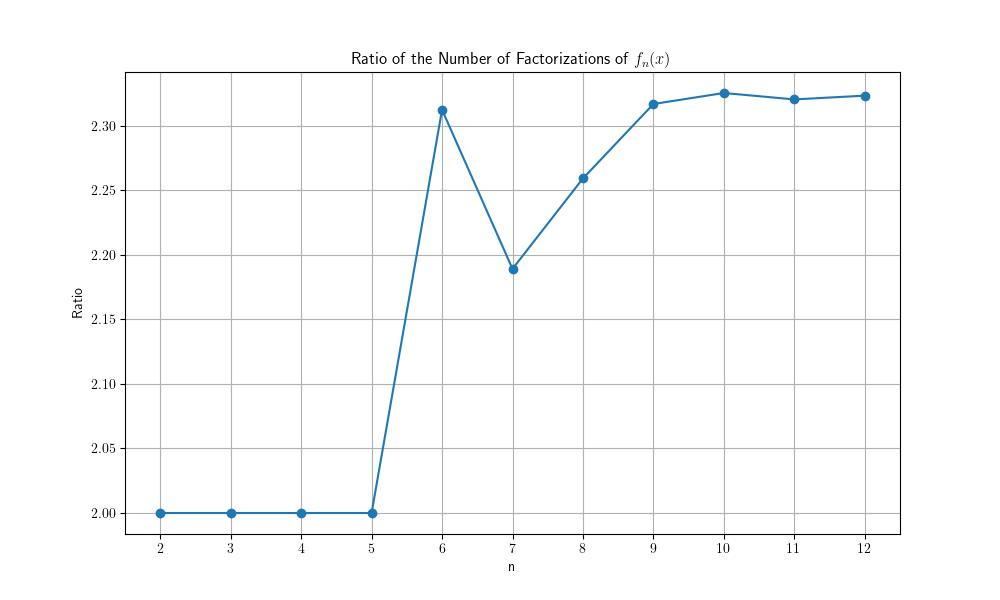
\includegraphics[width=0.75\textwidth]{ratio.jpg}
    \end{figure}

    \begin{table}[h!]
            \centering
            \caption{Number of unique factorizations}
            \label{tab:data}    
        \begin{tabular}{|r|r|r|}
            \hline
            $n$ & $2^{n+1}-1$ & \# factorizations \\ \hline
            1 & 3 & 1 \\ \hline 
            2 & 7 & 1 \\ \hline 
            3 & 15 & 2 \\ \hline 
            4 & 31 & 4 \\ \hline 
            5 & 63 & 8 \\ \hline 
            6 & 127 & 16 \\ \hline 
            7 & 255 & 37 \\ \hline 
            8 & 511 & 81 \\ \hline 
            9 & 1023 & 183 \\ \hline 
            10 & 2047 & 424 \\ \hline 
            11 & 4095 & 986 \\ \hline 
            12 & 8191 & 2288 \\ \hline 
            13 & 16383 & 5316 \\ \hline 
        \end{tabular}

    \end{table}
    
    \begin{table}[h!]
    \centering
    \caption{Unique Factorizations by number of irreducible factors}
    \label{tab:data}
    \begin{tabular}{|l|*{14}{r|}}
        \hline
        $n$  & $2^{n+1}-1$ & 1 & 2 & 3 & 4 & 5 & 6 & 7 & 8 & 9 & 10 & 11 & 12 & 13 \\
        \hline
        1  & 3 & 1 & & & & & & & & & & & & \\
        \hline
        2  & 7 & & 1 & & & & & & & & & & & \\
        \hline
        3  & 15 & & 1 & 1 & & & & & & & & & & \\
        \hline
        4  & 31 & & 2 & 1 & 1 & & & & & & & & & \\
        \hline
        5  & 63 & & 2 & 4 & 1 & 1 & & & & & & & & \\
        \hline
        6  & 127 & & 3 & 7 & 4 & 1 & 1 & & & & & & & \\
        \hline
        7  & 255 & & 6 & 16 & 9 & 4 & 1 & 1 & & & & & & \\
        \hline
        8  & 511 & & 11 & 33 & 22 & 9 & 4 & 1 & 1 & & & & & \\
        \hline
        9  & 1023 & & 18 & 75 & 51 & 24 & 9 & 4 & 1 & 1 & & & & \\
        \hline
        10  & 2047 & & 42 & 162 & 125 & 56 & 24 & 9 & 4 & 1 & 1 & & & \\
        \hline
        11 & 4095 & & 84 & 373 & 290 & 142 & 58 & 24 & 9 & 4 & 1 & 1 & & \\
        \hline
        12 & 8191 & & 179 & 833 & 696 & 336 & 147 & 58 & 24 & 9 & 4 & 1 & 1 & \\
        \hline
        13 & 16383 & & 385 & 1888 & 1613 & 833 & 351 & 149 & 58 & 24 & 9 & 4 & 1 & 1 \\
        \hline
    \end{tabular}
\end{table}

\pagebreak
\section{Future work}
Related future topics could include:
\begin{itemize}
    \item Establishing better upper and lower bounds for the number of factorizations of $f_n(x)$.
    \item Finding better criteria for determining when a polynomial is irreducible.
    \item Determining the number of factors of forms other than $(x + 1)h(x) = f_n(x)$.
    
    \begin{itemize}
        \item We suspect $(x^k + 1)h(x) = f_n(x)$ is a good class of candidates for making similar arguments.
    \end{itemize}
    \item General improvements such as faster algorithms.
\end{itemize}

\pagebreak
\bibliographystyle{apacite}
\bibliography{ref}
\nocite{*}

\end{document}
